%===============================================================================
\section{Description des distributions scientifiques}
%_______________________________________________________________________________
%...............................................................................
\begin{frame}[fragile]
\frametitle{Principales Distributions Scientifiques}
\begin{itemize}
 \item Numpy : essentielle en calcul numérique. 
 \item Matplotlib, Pylab : tracé de figures et fonctions à la matlab.  
 \item Scipy : outils scientifiques spécifiques.  
 \item Maiavi : 3D avancée. 
\end{itemize}
\end{frame}
%...............................................................................
\subsection{Numpy}
%...............................................................................
\begin{frame}[fragile]
\frametitle{Numpy}
\begin{itemize}
 \item \myFig{height=0.5cm}{./fig/numpy-logo.png} : \url{http://www.numpy.org}
 \item \emph{NumPy is the fundamental package for scientific computing with Python}
 \item Création d'objets ndarray.
 \item ndarray créés à partir de listes. 
 \item Accès aux éléments : A[i, j]
\end{itemize}
\begin{pythonConsole}
>>> import numpy as np
>>> A = np.array([1, 5, 2, 4, 3])
>>> type(A)
<type 'numpy.ndarray'>
>>> A.dtype
dtype('int32')
>>> A = np.array([[1., 2, 3], [4, 5, 6], [7, 8, 9.]])
>>> A[0, 0]
1.0
>>> A[2, 2]
9.0
\end{pythonConsole}
\end{frame}

% 
% frame
%

\begin{frame}[fragile]
\frametitle{Numpy}
\framesubtitle{Tableaux ND et fonctions associ\'ees}

\begin{itemize}
 \item Les exemples sont donnés dans IPython avec les fonctions Pylab chargées.  
\end{itemize}

\begin{pythonConsole}
>>> A = array([[1,2,3],[4,5,6],[7,8,9]])
>>> whos

Variable   Type       Data/Info
-------------------------------
A          ndarray    3x3: 9 elems, type `int64`, 72 bytes

>>> A
array([[1, 2, 3],
       [4, 5, 6],
       [7, 8, 9]])
       
>>> A.size
9

>>> A.shape
(3,3)

>>> B = array([[1,0,0],[0,1,0],[0,0,1]])

>>> A*B

array([[ 1.,  0.,  0.],
       [ 0.,  5.,  0.],
       [ 0.,  0.,  9.]])
\end{pythonConsole}
\end{frame}

% 
% frame
% 

\begin{frame}
\frametitle{Numpy}
\framesubtitle{Tableaux ND et fonctions associ\'ees}
$\bullet$ M\'ethodes
\begin{itemize}
\item nonzero, max, min, mean, std ...
\item sum, cumprod, cumsum ...
\item reshape, resize, flatten, transpose ... 
\end{itemize}
\vspace{0.5cm}
$\bullet$ Fonctions
\begin{itemize}
\item $*$ : produit \'elt./\'elt.
\item $dot(.,.)$ : produit matriciel
\item ...
\end{itemize}
\end{frame}
%
% frame
%
\begin{frame}[fragile]
\frametitle{Numpy}
\framesubtitle{NDarray {\em vs.} matrix}
\begin{pythonConsole}
>>> A = array([[1.,2,3],[4,5,6],[7,8,9]])
>>> B = array([[1,0,0],[0,1,0],[0,0,1]])
>>> C = matrix([[1.,2,3],[4,5,6],[7,8,9]])
>>> D = matrix([[1,0,0],[0,1,0],[0,0,1]])

>>> whos
Variable   Type       Data/Info
-------------------------------
A          ndarray    3x3: 9 elems, type `float64`, 72 bytes
B          ndarray    3x3: 9 elems, type `int64`, 72 bytes
C          matrix     [[ 1.  2.  3.]\n [ 4.  5.  6.]\n [ 7.  8.  9.]]
D          matrix     [[1 0 0]\n [0 1 0]\n [0 0 1]]

>>> dot(A,B)

array([[ 1.,  2.,  3.],
       [ 4.,  5.,  6.],
       [ 7.,  8.,  9.]])

>>>  C*D

matrix([[ 1.,  2.,  3.],
        [ 4.,  5.,  6.],
        [ 7.,  8.,  9.]])

\end{pythonConsole}
\end{frame}

% 
% Slide
% 

\begin{frame}[fragile]
\frametitle{Numpy}
\framesubtitle{matrix}
$\bullet$ M\'ethodes
\begin{itemize}
\item min, max, mean, std, ...
\item .T, .H, .I, ...
\item reshape, flatten, ...
\end{itemize}
\vspace{0.2cm}
$\bullet$ Fonctions
\begin{itemize}
\item inv, svd, eig, ...
\end{itemize}
\vspace{0.2cm}
\underline{Diff\'erences entre array et matrix}
\begin{pythonConsole}
>>> A = array([[1.,2,3],[4,5,6],[7,8,9]])
>>> B = matrix([[1.,2,3],[4,5,6],[7,8,9]])

>>> A**2
array([[  1.,   4.,   9.],
       [ 16.,  25.,  36.],
       [ 49.,  64.,  81.]])

>>> B**2
matrix([[  30.,   36.,   42.],
        [  66.,   81.,   96.],
        [ 102.,  126.,  150.]])

\end{pythonConsole}
\end{frame}
%...............................................................................
%
% frame
%
%...............................................................................
\begin{frame}[fragile]
\frametitle{Numpy}
\framesubtitle{NDarray {\em vs.} matrix}
\begin{pythonConsole}
>>> A = array([[1.,2,3],[4,5,6],[7,8,9]])
>>> B = array([[1,0,0],[0,1,0],[0,0,1]])
>>> C = matrix([[1.,2,3],[4,5,6],[7,8,9]])
>>> D = matrix([[1,0,0],[0,1,0],[0,0,1]])

>>> whos
Variable   Type       Data/Info
-------------------------------
A          ndarray    3x3: 9 elems, type `float64`, 72 bytes
B          ndarray    3x3: 9 elems, type `int64`, 72 bytes
C          matrix     [[ 1.  2.  3.]\n [ 4.  5.  6.]\n [ 7.  8.  9.]]
D          matrix     [[1 0 0]\n [0 1 0]\n [0 0 1]]

>>> dot(A,B)

array([[ 1.,  2.,  3.],
       [ 4.,  5.,  6.],
       [ 7.,  8.,  9.]])

>>>  C*D

matrix([[ 1.,  2.,  3.],
        [ 4.,  5.,  6.],
        [ 7.,  8.,  9.]])

\end{pythonConsole}
\end{frame}
%...............................................................................
%
% frame
%
%...............................................................................
\begin{frame}[fragile]
\frametitle{Numpy}
\framesubtitle{matrix}
$\bullet$ M\'ethodes
\begin{itemize}
\item min, max, mean, std, ...
\item .T, .H, .I, ...
\item reshape, flatten, ...
\end{itemize}
\vspace{0.2cm}
$\bullet$ Fonctions
\begin{itemize}
\item inv, svd, eig, ...
\end{itemize}
\vspace{0.2cm}
\underline{Diff\'erences entre array et matrix}
\begin{pythonConsole}
>>> A = array([[1.,2,3],[4,5,6],[7,8,9]])
>>> B = matrix([[1.,2,3],[4,5,6],[7,8,9]])

>>> A**2
array([[  1.,   4.,   9.],
       [ 16.,  25.,  36.],
       [ 49.,  64.,  81.]])

>>> B**2
matrix([[  30.,   36.,   42.],
        [  66.,   81.,   96.],
        [ 102.,  126.,  150.]])

\end{pythonConsole}
\end{frame}
%...............................................................................
%_______________________________________________________________________________
%_______________________________________________________________________________
\subsection{Matplotlib}
%...............................................................................
\begin{frame}[fragile]
\frametitle{Matplotlib}
\framesubtitle{Librairie graphique}
\begin{itemize}
\item Outils graphiques 2D
\item Toolkits : Basemap, Axesgrid, mplot3d
\item Beaucoup d'exemples : www.matplotlib.org
\end{itemize}
\begin{minipage}{0.68\linewidth}
\begin{pythonConsole}
>>> t=arange(0,1,10e-5)
>>> S1=sin(2*pi*2*t);S2=sin(2*pi*7*t+(3*pi/7)),
>>> fig=figure()
>>> ax=fig.add_subplot(111,xlim=(-1,1),ylim=(-1,1))
>>> courbe=ax.plot(S1,S2);ax.grid('on')
>>> annotate('Courbe',xy=(-0.5,0.5),xytext=(-0.65,0),\
       bbox=dict(boxstyle='round,pad=0.5',fc='red',\ 
       alpha=0.2),arrowprops=dict(arrowstyle='->',\
         connectionstyle='arc3,rad=0'))
>>> title(r"Figure de Lissajous ($\nu_1=2$, $\nu_2=1$,\
         $\phi=\frac{3\pi}{7}$)")
>>> xlabel(r"$\sin(2\pi\nu_1 t)$")
>>> ylabel(r"$\sin(2\pi\nu_2 t + \phi)$")
>>> show()

\end{pythonConsole}
\end{minipage}
\begin{minipage}{0.3\linewidth}
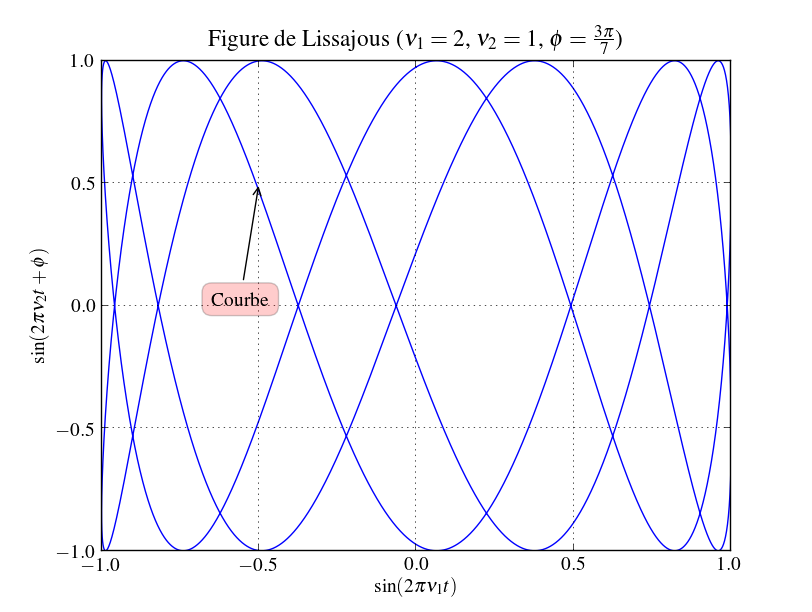
\includegraphics[width=4.5cm,height=4.5cm]{fig/Lissajous.png}
\end{minipage}
\end{frame}

% 
% Slide
% 

\begin{frame}[fragile]
\frametitle{Matplotlib}
\framesubtitle{Exemples}
\begin{minipage}{0.58\linewidth}
\begin{pythonConsole}
>>> [X,Y] = meshgrid(linspace(-2,2,500),\
linspace(-2,2,500))
>>> Z=X+Y*1j
>>> k=1
>>> while k<=75:
>>> 	Z = Z - (Z/3 - 1) / (3*Z**2)
>>>	k=k+1
>>> close('all')	
>>> imshow(angle(Z),cmap=cm.gray)
>>> #savefig('/MonChemin/Lenom.pdf',format='pdf')
>>> show()
\end{pythonConsole}
\end{minipage}
%\hspace{0.5cm}
\begin{minipage}{0.4\linewidth}
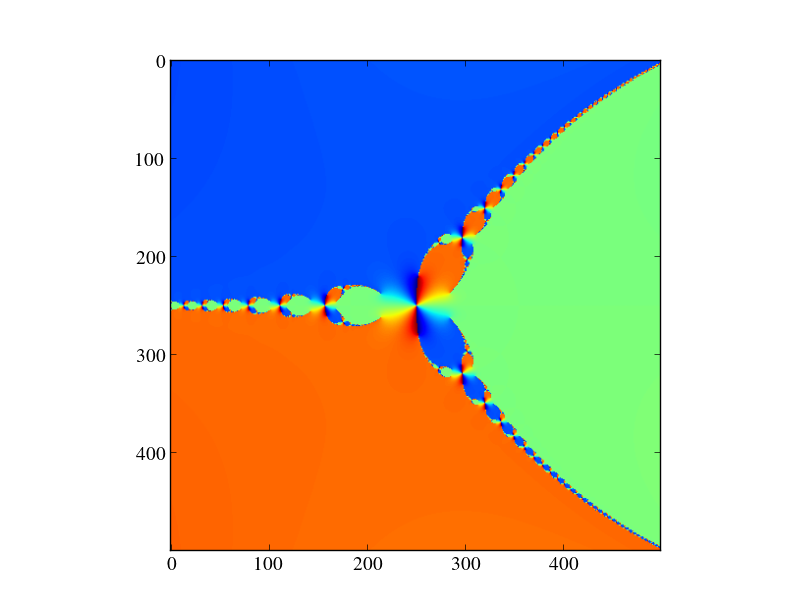
\includegraphics[width=5.5cm,height=4.5cm]{fig/fractal.png}
\end{minipage}
\end{frame}

% 
% Slide
% 
\begin{frame}
\frametitle{Matplotlib}
\framesubtitle{Exemples}

\begin{minipage}{0.4\linewidth}
\begin{figure}
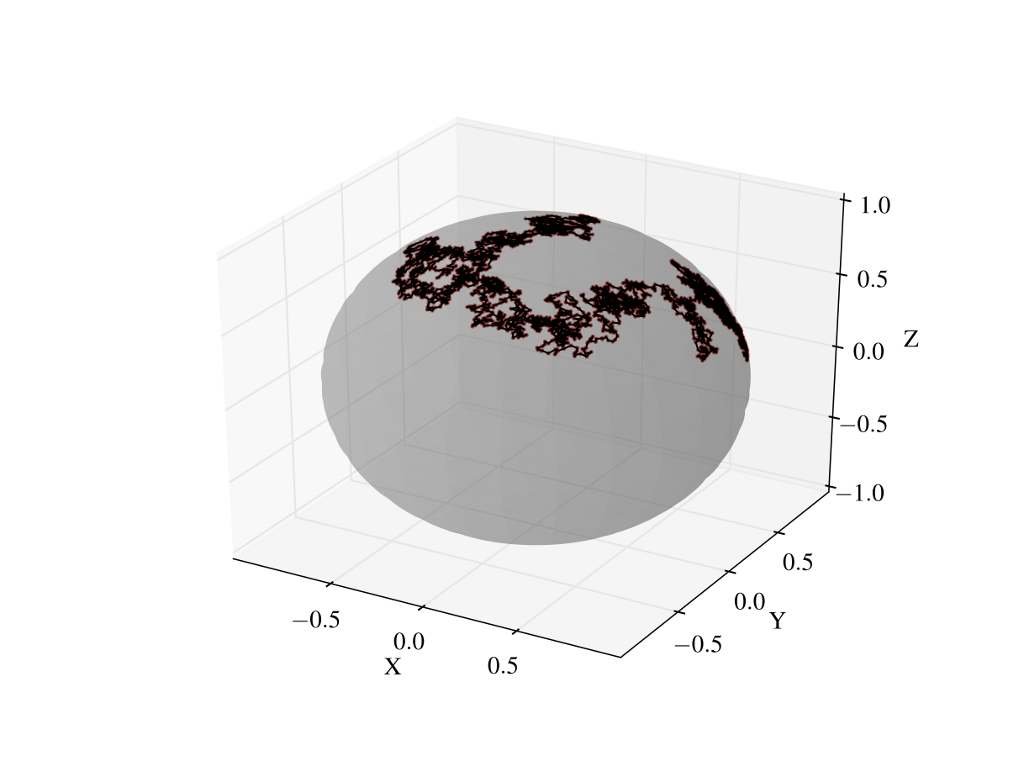
\includegraphics[width=6.5cm,height=5.5cm]{fig/BrownSphere.png}
\end{figure}
\end{minipage}
\hspace{1cm}
\begin{minipage}{0.4\linewidth}
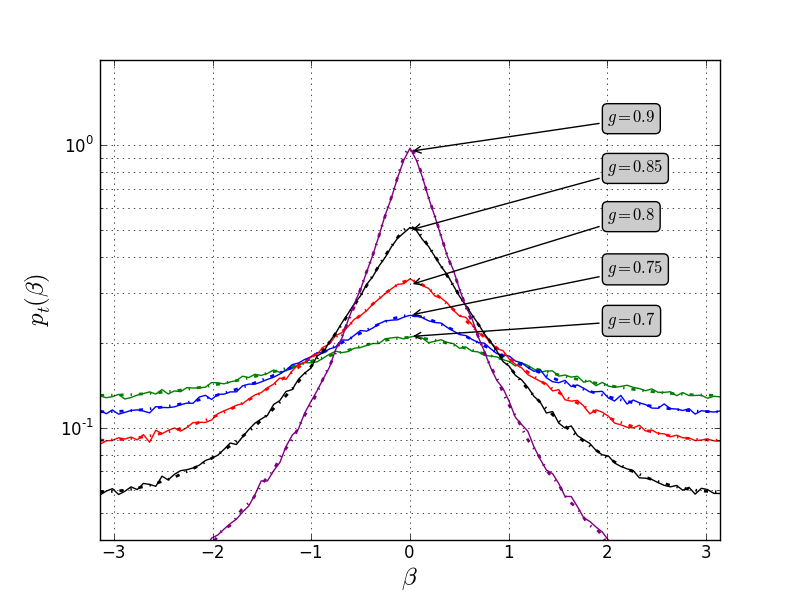
\includegraphics[width=5.5cm,height=4.5cm]{fig/Distrib.png}
\end{minipage}
\end{frame}
%...............................................................................
%_______________________________________________________________________________
%_______________________________________________________________________________
\subsection{Pylab}
%...............................................................................
\begin{frame}[fragile]
\frametitle{Pylab}
\framesubtitle{}
\begin{itemize}
 \item Module de Matplotlib : matplotlib\slash{}pylab.py
 \item Redéfinit des fonctions à la Matlab.
 \item Raccourci : "import pylab" au lieu de "import matplotlib.pylab"
 \item En général, et exceptionnellement, s'utilise : "from pylab import *" 
\end{itemize}
\begin{pythonConsole}
>>> from pylab import *
>>> plot([1, 5, 2, 4, 3])
[<matplotlib.lines.Line2D object at 0x4ec05b0>]
>>> show()
>>> a = randn(100, 10)
>>> type(a)
<type 'numpy.ndarray'>
>>> a.shape
(100, 10)
>>> help(matplotlib.pylab)
\end{pythonConsole}
\end{frame}
%...............................................................................
%_______________________________________________________________________________
%_______________________________________________________________________________
\subsection{Scipy}
%...............................................................................
\begin{frame}
\frametitle{Scipy}
\framesubtitle{Scientific library}
\begin{itemize}
 \item \myFig{height=0.5cm}{./fig/scipy-logo.png}\ : http://www.scipy.org 
\end{itemize}
\begin{center}
\tiny
\begin{tabular}{p{3cm}p{2cm}|p{3cm}p{2cm}}
Clustering package & scipy.cluster & Constants & scipy.constants \\
Discrete Fourier transforms & scipy.fftpack & Integration and ODEs & scipy.integrate \\
Interpolation & scipy.interpolate & Input and output & scipy.io \\
Linear algebra & scipy.linalg & Miscellaneous routines & scipy.misc \\
Multi-dimensional image processing & scipy.ndimage & Orthogonal distance regression & scipy.odr \\
Optimization and root finding & scipy.optimize & {\bfseries Signal processing} & scipy.signal \\
Sparse matrices & scipy.sparse & Sparse linear algebra & scipy.sparse.linalg \\
Compressed Sparse Graph Routines & scipy.sparse.csgraph & Spatial algorithms and data structures & scipy.spatial \\
Special functions & scipy.special & Statistical functions & scipy.stats \\
Statistical functions for masked arrays & scipy.stats.mstats & 
C/C++ integration & scipy.weave \\
\end{tabular}
\end{center}
\end{frame}
%...............................................................................
%_______________________________________________________________________________
%_______________________________________________________________________________
\subsection{Mayavi}
%...............................................................................
\begin{frame}
\frametitle{Mayavi}
\framesubtitle{}
\frameCC{%
\begin{itemize}
 \item Manipulation des objets 3D améliorée. 
\end{itemize}
}
{\myFig{width=9cm}{./fig/Mayavi.png}}
\end{frame}
%...............................................................................
%...............................................................................
\begin{frame}[fragile]
\frametitle{Mayavi}
\framesubtitle{import mayavi.engine}
\begin{itemize}
 \item Dans une console Python : import mayavi. \dots
\end{itemize}
\begin{pythonConsole}
>>> from numpy import array
>>> from mayavi.api import Engine
>>> engine = Engine()
>>> engine.start()
>>> engine.new_scene()
>>> from mayavi.sources.parametric_surface import ParametricSurface
>>> parametric_surface1 = ParametricSurface()
>>> scene = engine.scenes[0]
>>> engine.add_source(parametric_surface1, scene)
>>> from mayavi.modules.surface import Surface
>>> surface1 = Surface()
>>> engine.add_filter(surface1,parametric_surface1)
\end{pythonConsole}
\end{frame}
%...............................................................................
%_______________________________________________________________________________
%_______________________________________________________________________________
\subsection{Autres ressources : exemple C}
%...............................................................................
\begin{frame}[fragile]
\frametitle{Importation de bibliothèques de fonction écrites en C}
\framesubtitle{Exemple using module ctypes}
\begin{python}
import ctypes

myLib = ctypes.LoadLibray('myLib.lib')
fun_c = myLib.fun 
fun_c.argtypes = [ctypes.c_double, ctypes.c_int]
fun_c.restype = ctypes.c_int (default)

n = len(s)
pathFile = os.path.dirname(__file__)
libName = os.path.join(pathFile, 'clz.lib')
print('libName + ' + libName)
libCLZ = ctypes.CDLL(libName)
clz_c = libCLZ.clz
clz_c.restype = ctypes.c_uint
sequence = numpy.ctypeslib.ndpointer(dtype=numpy.int) 
clz_c.argtypes = ([sequence, ctypes.c_uint])
# conversion of s into sequence with numpy.asarray
c = clz_c(numpy.asarray(s, dtype='int'), n)
\end{python}
\end{frame}
%...............................................................................
\hide{%
%...............................................................................
\begin{frame}
\frametitle{Cython}
pas vu \dots
\end{frame}
%...............................................................................
}
\hide{%
%...............................................................................
\begin{frame}
\frametitle{Fortran to Python}
\framesubtitle{f2p}
Gestion des modules fortran cf Lapack 'f2p'. 

Importation comme les fonctions python import a.fun. 

En cours d'évaluation. 
\end{frame}
%...............................................................................
}
%_______________________________________________________________________________
%===============================================================================

%%% Local Variables: 
%%% mode: latex
%%% TeX-master: "presentationPython"
%%% End: 
